% Chapter 4

\chapter{Sentiment Analysis using Topic models} % Main chapter title

\label{topicmodeledsa} % For referencing the chapter elsewhere, use \ref{Chapter4} 

\lhead{Chapter 4. \emph{Sentiment Analysis using Topic models}} % This is for the header on each page - perhaps a shortened title

%----------------------------------------------------------------------------------------

In this chapter, we will show how topic models are used for \textit{SA}. In the first section, we go through some of the related work where sentiment and topic have
been jointly modeled. After that, we show how the basic \textit{LDA} model can be used  to classify documents based on their polarity.  This is followed by the 
explanation of the \textit{JST} model in detail. The use of \textit{Topical n-grams} model for \textit{SA} is shown in the section following this. The experimental
setup, results, and error analysis is done in ~\sref{experiments}.

Joint sentiment and topic models have been used to tackle the sentiment classification problem. Despite having a hierarchical structure, these generative models have 
a bag of words assumption. Due to this fact, they tend to misclassify texts having sentiment in the form of phrases. \textit{LDA} and it's extensions don't work properly
with phrases. To tackle this situation, we propose an unsupervised approach to sentiment analysis using the topical n-grams model which has been shown to be effective 
with phrases. We train the topical n-grams model using two topics i.e., positive, and negative, list of positive and negative words, and rules to detect positive and 
negative phrases. New documents are then classified using this trained model. The system gives better results than the existing Joint Sentiment Topic model. We also propose
an approach to generate a list of positive and negative words using LDA based on our observations reported in ~\sref{experiments}.

In the next section, we will point out some of the related work in this direction.

\section{Related Work}

There are many supervised, semi-supervised and unsupervised approaches to solve the sentiment analysis problem. One supervised method based on n-gram analysis is explained
by \citep*{bespalov2011sentiment}. In this they map the n-grams to a low-dimensional latent semantic space where a classification function can be defined. Our approach being
unsupervised, we will go through some of the related work in that direction. One more motivation to consider only semi-supervised and unsupervised approaches is the fact that
they don't need any corpus and don't have any domain specific limitations. Rule based systems can also be considered as unsupervised systems but usually due to exceptions to
these rules, their performance is affected. Due to this, we are not considering them in further discussion.

\citep*{turney2002thumbs} used an unsupervised learning algorithm based on mutual information between document phrases and a small set of positive/negative paradigm words 
called seed words to classify the semantic orientation at the word/phrase level. Another unsupervised approach to classify the text at document level was proposed by \citep*{turney2002unsupervised}. 
\citep*{eguchi2006sentiment} created a generative model that jointly models sentiment words, topic words and sentiment polarity in a sentence as a triple. \citep*{mei2007topic} 
proposed another generative model, called TSM (Topic Sentiment Mixture) model which can be used to discover topics in blogs as well as their associated sentiments. A novel 
generation model that unifies topic-relevance and opinion generation by a quadratic combination was proposed by \citep*{zhang2008generation}. A probabilistic generative model 
based on LDA called JST (Joint Sentiment Topic) model was shown to perform well for sentiment analysis of reviews by \citep*{lin2009joint}. It is a fully unsupervised method
and shows good result when priors are used for training. Another extension of LDA which tries to unify aspect and sentiment was proposed by \citep*{jo2011aspect}. All the 
unsupervised methods using generative models discussed here operate at the word level. Due to this they lose out on the information provided by phrases which may lead to 
incorrect classification.

In the next section, we will show how to use the basic \textit{LDA} model for sentiment analysis.

\section{LDA for sentiment analysis}

Let us first list the basic steps to use any topic model for discovering topics.

\subsection{Using Topic models}

\begin{itemize}
 \item Set number of topics.
 \item Remove stop-words as they do not belong to any topic.
 \item Estimate probabilities using some inference method.
 \item Use the trained model for inference of topics in new documents.
\end{itemize}

\subsection{Using LDA for Sentiment Classification}

To use basic LDA as a sentiment classifier, we add one more step to remove objective words. Also, usually during Gibbs sampling the first step assigns topics 
randomly to words. Instead, we introduce a prior information about the positivity and negativity of words to assign topics to words initially. The steps are 
as follows.

\begin{itemize}
 \item Set number of topics, 2 in this case viz. positive and negative.
 \item Remove stop-words.
 \item Remove objective words as they won't affect sentiment.
 \item \textbf{Gibbs Sampling} with prior using lists of positive and negative words.
  Gibbs Sampling was explained in detail in \cref{ir}. We will again explain it briefly here.
  \begin{itemize}
   \item Go through each document, and randomly assign each word in the document to one of the \(K\) topics. this random assignment already gives you both topic 
   representations of all the documents and word distributions of all the topics (albeit not very good ones). 
   \item So to improve on them, for each document \(d\), go through each word \(w\) in \(d\), and for each topic \(t\), compute two things.
   \begin{enumerate}
    \item \(p(t|d)\) = the proportion of words in document \(d\) that are currently assigned to topic \(t\).
    \item \(p(w|t)\) = the proportion of assignments to topic \(t\) over all documents that come from this word \(w\). 
   \end{enumerate}
   \item After this, Reassign \(w\) a new topic, where you choose topic \(t\) with probability \(p(t|d) \times p(w|t)\) . According to the generative model, this is 
   essentially the probability that topic \(t\) generated word \(w\), so it makes sense that we re-sample the current word's topic with this probability. In this step,
   we're assuming that all topic assignments except for the current word in question are correct, and then updating the assignment of the current word using our model 
   of how documents are generated.
   \item After a suitable number of iterations, we get a proper probability distribution.
  \end{itemize}
  As explained here, the \textbf{first step assigns topics randomly}. In our case, we make \textbf{use of prior knowledge which a list of positive and negative words
  to assign the positive or negative topic to each word} initially. The inclusion of prior increases the accuracy of the system as shown in ~\sref{experiments}.
 \item Use the trained model to classify a new document as positive or negative.
\end{itemize}

Having prior knowledge in the case of LDA, means we have the word-topic distribution as shown in Figure 4.1.

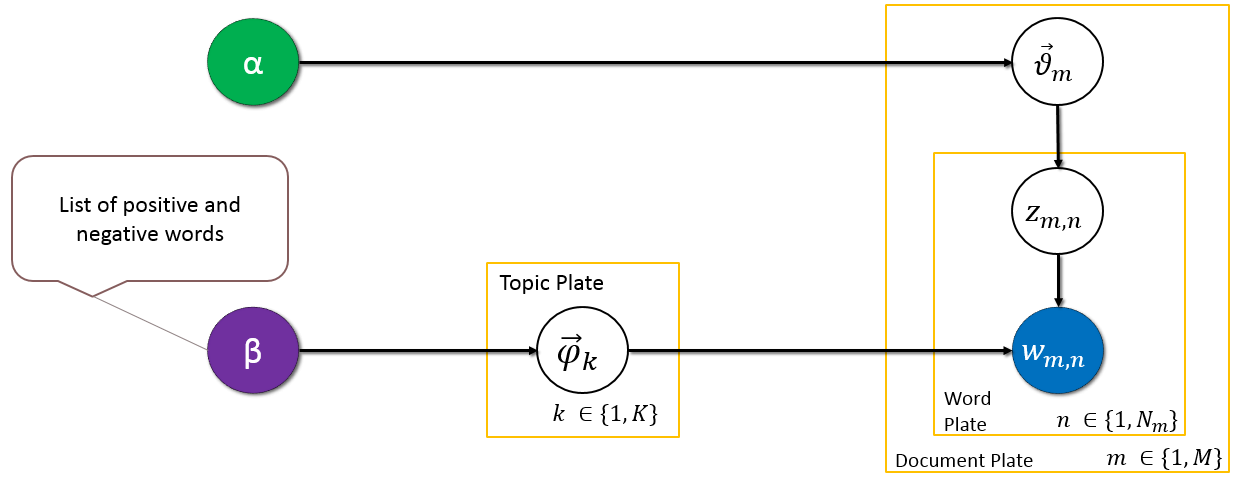
\includegraphics[width=\textwidth]{lda/ldawithprior.png} 
\begin{center}
 Figure 4.1 LDA with prior
\end{center}

\subsection{Example}

Let us consider an example to see how it works. 

\textbf{Text Input}

\textit{ Okay, so Janet is an AMAZING actress, I love her brother MJ so thats why I rented this. I was amazed at the emotion she put into her character, this 
movie is NOT for young children! She did amazing channeling the anger that Patricia had to potray, I think this is a MUST SEE movie!}

\textbf{After converting to lower case}

\textit{ okay, so janet is an amazing actress, i love her brother mj so thats why i rented this. i was amazed at the emotion she put into her character, this 
movie is not for young children ! she did amazing channeling the anger that patricia had to potray, i think this is a must see movie!}

\textbf{After removing stop-words}

\textit{ {\color[rgb]{0.4,0.4,0.4}okay, so} janet {\color[rgb]{0.4,0.4,0.4}is an} amazing actress, {\color[rgb]{0.4,0.4,0.4}i} love {\color[rgb]{0.4,0.4,0.4}her}
brother mj {\color[rgb]{0.4,0.4,0.4}so thats why i} rented {\color[rgb]{0.4,0.4,0.4}this}. {\color[rgb]{0.4,0.4,0.4}i was} amazed {\color[rgb]{0.4,0.4,0.4}at the}
emotion {\color[rgb]{0.4,0.4,0.4}she put into her} character, {\color[rgb]{0.4,0.4,0.4}this} movie {\color[rgb]{0.4,0.4,0.4}is not for} young children ! 
{\color[rgb]{0.4,0.4,0.4}she did} amazing channeling {\color[rgb]{0.4,0.4,0.4}the} anger {\color[rgb]{0.4,0.4,0.4}that} patricia {\color[rgb]{0.4,0.4,0.4}had to} 
potray, {\color[rgb]{0.4,0.4,0.4}i} think {\color[rgb]{0.4,0.4,0.4}this is a} must {\color[rgb]{0.4,0.4,0.4}see} movie!}

\textbf{After removing objective words}

\textit{ {\color[rgb]{0.4,0.4,0.4}okay, so janet is an} amazing {\color[rgb]{0.4,0.4,0.4}actress, i} love {\color[rgb]{0.4,0.4,0.4}her brother mj so thats why i rented 
this. i was} amazed {\color[rgb]{0.4,0.4,0.4}at the emotion she put into her character, this movie is not for young children ! she did} amazing {\color[rgb]{0.4,0.4,0.4}channeling 
the} anger {\color[rgb]{0.4,0.4,0.4}that patricia had to potray, i think this is a must see movie! }}

\textbf{After assigning topic to each subjective word using the word lists}

\textit{ {\color[rgb]{0.4,0.4,0.4}okay, so janet is an} {\color{green}amazing} {\color[rgb]{0.4,0.4,0.4}actress, i} {\color{green}love} {\color[rgb]{0.4,0.4,0.4}her 
brother mj so thats why i rented this. i was} {\color{green}amazed} {\color[rgb]{0.4,0.4,0.4}at the emotion she put into her character, this movie is not for young 
children ! she did} {\color{green}amazing} {\color[rgb]{0.4,0.4,0.4}channeling the} {\color{red}anger} {\color[rgb]{0.4,0.4,0.4}that patricia had to potray, i think 
this is a must see movie! }}

After this the Gibbs sampling procedure is performed on the input text. The final outcome depends on the counts of positive and negative words in the document. But as the 
sampling procedure ensures that co-occuring words belong to the same topic, the system performs well in many cases as can be seen in the experimental results shown in
~\sref{experiments}. This is similar to the bag of words model where the feature vector contains only subjective words.

In the next two sections, we will go through the joint models of topic and sentiment.

\section{Joint models of topic and sentiment}

SA has been used in IR to improve the performance. IR was mainly concerned with factual/objective data. So, intuitively we see that subjectivity classification 
can aid IR. \citep*{riloff2005exploiting} has work based on it in which they try to exploit subjectivity analysis to improve performance of information extraction. 

Corpus models are useful in fetching documents specific to a certain topic. Sometimes a user might need to fetch documents which have a specific sentiment. One 
such work on sentiment retrieval using generative models is seen in \citep*{eguchi2006sentiment}. In this work, they have assumed that user inputs both query 
terms as well as indicates the desired sentiment polarity in some way. They have combined sentiment and topic relevance models to retrieve documents which are most
relevant to such user requests. This approach is very important for sentiment aware information retrieval.

The expression of sentiment in the text is topic dependent. Negative review for a voting event may be expressed using \textit{flawed}. On the other hand negative 
review of politician may be expressed using \textit{reckless}. Sentiment polarity is topic dependent \citep*{engstrom2004topic}. The adjective \textit{unpredictable}
will have a negative orientation in a car review and it will have a positive orientation in a movie review. 

\subsection{Terminology}

The goal of the model is to generate a collection of sentences \(s_1,s_2,\dots,s_n\). Every document is composed of words \(w_1,w_2,\dots,w_n\) drawn from the vocabulary
\(V\). A binary variable \(b_{ij} \in \{S,T\}\) is used to represent whether a word in position \(j\) in sentence \(i\) is a topic word or a sentiment word. Let \(x_i\)
be the polarity for the sentence \(s_i\). \(x_i\) is a discrete random variable with three outcomes \(\{-1,0,+1\}\). A statement \(s_i\) is represented as a set 
\(\{w_i^s,w_i^t,x_i\}\) where \(w_i^s\) are the sentiment bearing words, \(w_i^t\) are the topic bearing words and \(x_i\) is the sentence polarity. The user query will
be represented in a similar fashion \(\{q_i^s,q_i^t,q^x\}\). Let \(p\) denote a unigram language model. \(P\) denotes the set of all possible language models. It is the
probability simplex. Similarly, let \(p_x\) denote the distribution over three possible polarity values and \(P_x\) will be the corresponding ternary probability simplex.
The function \(\pi:P \times P \times P_x\to[0,1]\) is a function which assigns a probability \(\pi(p_1,p_2,p_x)\) to a pair of language models \(p_1\) and \(p_2\) together
with \(p_x\).

\subsection{Generative model of sentiment}

A sentence \(s_i\) containing words \(w_1,w_2,\dots,w_j,\dots,w_m\) is generated in the following way:

\begin{enumerate}
 \item Draw \textit{p_t, p_s and p_x} from \(\pi (\cdot,\cdot,\cdot)\).
 \item Sample \(x_i\) from a polarity distribution \(p_x(\cdot)\).
 \item For each position \(\textit{j = 1\dots m}\):
  \begin{itemize}
   \item if \(b_{ij}=T\): draw \(w_{j}\) from \(p_t(\cdot)\);
   \item if \(b_{ij}=S\): draw \(w_{j}\) from \(p_s(\cdot)\)
  \end{itemize}
\end{enumerate}

The probability of observing the new statement \(s_i\) containing words \(w_1,w_2,\dots,w_j,\dots,w_m\) is given by:

\begin{equation}
\sum_{p_t,p_s,p_x} \pi(p_t,p_s,p_x)p_x(x_i) \prod_{j=1}^m \left\{ 
  \begin{array}{l l}
    p_t(w_j) & \quad \text{if b_{ij} = T}\\
    p_s(w_j) & \quad \text{otherwise}
  \end{array} \right.
\end{equation}

The probability functions are dirichlet smoothed models and \(\pi(p_1,p_2,p_x)\) is a non-parametric function. 

Each sentence is represented as a bag of words model and the model makes strong independence assumptions. But, due to joint probability distribution used it is able to
model co-occurrence. 

\subsubsection*{Retrieval using the model}

Suppose we are given a collection of statement \(C\) and a query \(\{q_i^s,q_i^t,q^x\}\) given by the user. The topic relevance model \(R_t\) and the sentiment relevance
model \(R_t\) are estimated. For each word \(w\) in a statement within a collection \(C\), these models are estimated as follows:


\begin{equation}
R_t(w) = \frac{P(q^s,q^t\circ w,q^x)}{P(q^s,q^t,q^x)} , R_s(w) = \frac{P(q^s \circ w,q^t,q^x)}{P(q^s,q^t,q^x)} 
\end{equation}

\(q \circ w\) means appending \(w\) to the list \(q\). The statements are ranked using a variation of cross-entropy,

\begin{equation}
 \alpha \sum_v R_t(v) \log p_t (v) + (1-\alpha) \sum_v R_s(v) \log p_s(v)
\end{equation}

\par

The experiments using this approach have shown promising results. This shows that sentiment aware IR can benefit from this technique. As corpus models have been widely 
used in IR, extending and tuning them for SA aware IR can yield good results. 


\subsection{Joint Sentiment-Topic modeling (JST)}

\citep*{lin2009joint} discusses a joint model of sentiment and topics. Following figure shows the model.

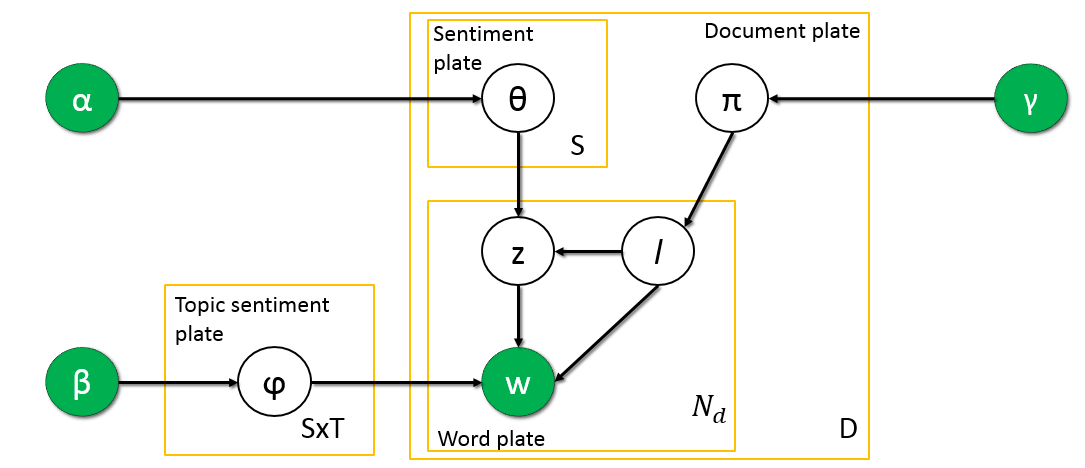
\includegraphics[width=\textwidth]{jst/jst2.png} 
\begin{center}
 Figure 4.2 Joint Sentiment Topic Model
\end{center}

Assume that we have a collection of \(D\) documents denoted by \(C = {d_1,d_2,\cdots,d_D} \); each document in the corpus is a sequence of \(N_d\) words denoted by 
\(d = (w_1,w_2,\cdots,w_{N_d}) \) and each word in the document is an item from a vocabulary index with V distinct terms denoted by \({1,2,\cdots,V}\). Let \(S\) and 
\(T\) be the number of distinct sentiment and topic labels respectively. The procedure of generating a document is described as follows.

\begin{alltt}
For each document \(d\), choose a distribution \(\pi_d \sim Dir(\gamma)\).
For each sentiment label \(l\) under document \(d\), choose a distribution
\(\theta_{d,k} \sim Dir(\alpha)\).
For each word \(w_i\) in document \(d\)
  - choose a sentiment label \(l_i \sim \pi_d\),
  - choose a topic \(z_i \sim \theta_{d,l_i}\),
  - choose a word \(w_i\) from the distribution over words defined by the 
    topic \(z_i\) and sentiment label \(l_i\), \(\psi_{z_i}^{l_i}\)
\end{alltt}

The hyper-parameter \(\alpha\) in \textit{JST} is the prior observation count for the number of times topic \(j\) is associated with  sentiment label \(l\) sampled from
a document. 

The hyper-parameter \(\beta\) is the prior observation count for the number of times words sampled from topic \(j\) are associated with sentiment label \(l\).

Similarly, the hyper-parameter \(\gamma\) is the prior observation count for the number of times sentiment label \(l\) is associated with a document.

The latent variables of interest in \textit{JST} are
\begin{enumerate}
 \item The joint sentiment/topic-document distribution, \(\theta\)
 \item The joint sentiment/topic-word distribution, \(\phi\)
 \item The joint sentiment-document distribution, \(\pi\)
\end{enumerate}

To obtain the distributions for \(\theta\), \(\phi\), and \(\pi\), we firstly estimate the posterior distribution over \(z\) i.e, the assignment of word tokens to
topics and sentiment labels.

We need to estimate the distribution, \(P(z_t=j,l_t=k|w,z_{\neg t},l_{\neg t},\alpha,\beta,\gamma)\) where \(z_{\neg t}\) and \(l_{\neg t}\) are vector of assignments
of topics and labels for all words in the collection except for the word position \(t\) in document \(d\). 

The joint distribution can be given as follows,
\begin{equation}
P(w,z,l) = P(w|z,l)P(z|l) = P(w|z,l)P(z|l,d)P(l|d)
\end{equation}

After calculations similar to \textit{LDA}, we get the following full conditional,

\begin{equation}
P(z_t=j,l_t=k|w,z_{\neg t},l_{\neg t},\alpha,\beta,\gamma) = 
\frac{\{N_{i,j,k}\}_{\neg t} + \beta}{\{N_{j,k}\}_{\neg t}+V\beta}.
\frac{\{N_{j,k,d}\}_{\neg t} + \alpha}{\{N_{k,d}\}_{\neg t}+T\alpha}.
\frac{\{N_{k,d}\}_{\neg t} + \gamma}{\{N_{d}\}_{\neg t}+S\gamma}
\end{equation}

where,

\(V\) is the size of the vocabulary \\
\(T\) is the number of topics \\
\(S\) is the total number of sentiment labels \\
\(D\) is the number of documents in the collection \\
\(N_{i,j,k}\) is the number of times word \(i\) appeared in topic \(j\) and with sentiment label \(k\) \\
\(N_{j,k}\) is the number of times words are assigned to topic \(j\) and sentiment label \(k\) \\
\(N_{j,k,d}\) is the number of times a word from document \(d\) has been associated with topic \(j\) and sentiment label \(k\) \\
\(N_{k,d}\) is the number of times sentiment label \(k\) has been assigned to some word tokens in document \(d\) \\
\(N_{d}\) is the total number of words in the collection \\

\par

\(\theta\), \(\phi\), and \(\pi\) can be estimated as follows

\begin{equation}
\phi_{i,j,k} = \frac{N_{i,j,k}+\beta}{N_{j,k}+V\beta}
\end{equation}

\begin{equation}
\theta_{j,k,d} = \frac{N_{j,k,d}+\alpha}{N_{k,d}+T\alpha}
\end{equation}

\begin{equation}
\pi_{k,d} = \frac{N_{k,d}+\gamma}{N_{d}+S\gamma}
\end{equation}

The Gibbs sampling procedure in this case is similar to that of \textit{LDA}. 

\par
\textit{JST} can be used for document level sentiment classification and topic detection simultaneously. \textit{Joint sentiment topic modeling} is completely unsupervised
as compared to existing approaches for sentiment classification. The performance of \textit{JST} on movie review classification is competitive compared to other supervised
approaches. \textit{JST} has been used in our experiments to compare it against our approaches for sentiment analysis as explained in \sref{experiments}.

LDA (Latent Dirichlet Allocation) as shown by \citep*{blei2003latent} is a generative model used to discover topics in a document collection. It gives two types of 
distributions as output, document-topic and word-topic distributions. The document-topic distribution gives the proportion of topics in each document and the word-topic
distribution gives the probability of a word being in each topic. LDA works on the principle of co-occurrence. It assumes that words tending to appear together belong 
to the same topic. JST (Joint Sentiment Topic) as explained by \citep*{lin2009joint} is a probabilistic generative model which extends LDA and discovers both sentiment
and topic simultaneously in a document collection. JST has shown promising results on binary sentiment classification. 

There are many extensions of the basic LDA model which try to combine both sentiment and topic to solve the problem of sentiment analysis. All these models including LDA
have one underlying assumption which makes them unsuitable for text classification purposes. They assume that each word is generated separately and independent of other
words. This is essentially the bag of words assumption. However, text being a sequence of words, the correct meaning of the text cannot be understood by merely capturing
co-occurrences. In addition to this, we also need to consider collocation of words. A phrase is a collocation of words which usually has more meaning than the individual 
words making up that phrase. There is a subtle difference between a phrase and collocation of words. Not all collocations of words can be considered as a phrase. We need
a model which takes into account phrases to completely understand the meaning of the text.

Topical n-grams model proposed by \citep*{wang2007topical} is one such generative model which takes into account not only co-occurrences but also collocations of words. It
also decides whether a particular collocation of words should be considered as a phrase or not. We train this model using 3 topics viz. positive, negative and objective, 
using a prior list of positive and negative words, and some rules to identify the subjective nature of phrases. The phrases in our experiments are restricted to bigrams. We
then use this trained model to infer the topic distribution for new documents. The topic having higher proportion is considered to be the class of the document.

In the next section, we will explain the topical n-grams model.

\section{Topical n-grams model}

n-gram phrases (or collocations) are fundamentally important in many areas of natural language processing (e.g., parsing, machine translation and information retrieval). 
Phrase as the whole carries more information than the sum of its individual components, thus it is much more crucial in determining the topics of document collections than
individual words \citep*{wang2005note}. However, most of the topic models assume that words are generated independently to each other, i.e., under the bag of words assumption.
The possible over complicacy caused by introducing phrases makes these topic models completely ignore them. It is true that these models with the bag of words assumption have
enjoyed a big success, and attracted a lot of interests from researchers with different backgrounds. A topic model considering phrases would be more useful in certain 
applications. Topical n-grams model is one such generative model. It's generative process is explained as follows,


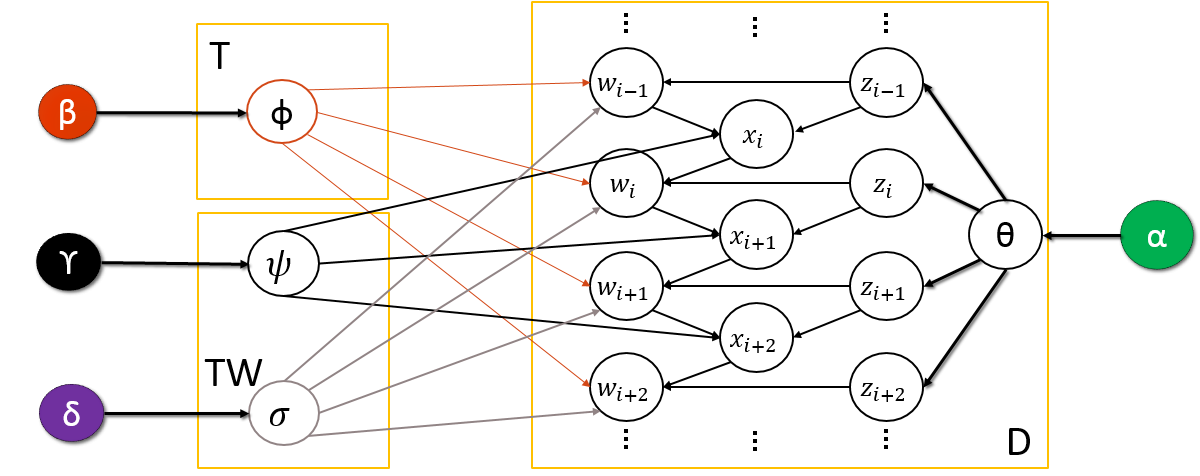
\includegraphics[width=\textwidth]{tng.png} 
\begin{center}
 Figure 4.3 Topical n-grams model
\end{center}

\begin{enumerate}
 \item Draw multinomial \(\phi_z\) from a Dirichlet prior \(\beta\);
 \item Draw binomial \(\psi_z\) from a Beta prior \(\gamma\);
 \item Draw multinomial \(\sigma_{zw}\) from a Dirichlet prior \(\delta\);
 \item For each document d, draw a multinomial \(θ^{(d)}\) from a Dirichlet prior \(\alpha\); then for each word \({w_i}^{(d)}\) in document \(d\),
    \begin{enumerate}
     \item Draw \({x_i}^{(d)}\) from binomial \(\psi_{{w_{i-1}}^{(d)}}\);
     \item Draw \({z_i}^{(d)}\) from multinomial \(\theta_{(d)}\);
     \item Draw \({w_i}^{(d)}\) from multinomial \(\sigma_{{w_{i-1}}^{(d)}}\) if \({x_i}^{(d)} = 1\); else draw \({w_i}^{d}\) from multinomial \(\phi_{{z_i}^{(d)}}\).
    \end{enumerate}
\end{enumerate}

The main point to infer from this generative process is that the topic assignments for the two terms in a bigram are not required to be identical. In the description of
topic n-grams given in \citep*{wang2005note}, they have used the topic of the last term as the topic of the phrase. But in our experiments, we have used certain rules
as prior information to assign topics to a phrase initially.

\subsection{Inferencing}

Gibbs sampling is used to conduct approximate inference in this paper. During Gibbs sampling, we draw the topic assignment \(z_i\) and the bigram status \(x_i\) iteratively
for each word \(w_i\) according to the following conditional probability distribution:

\begin{equation}
p(z_i,x_i | z_{-i},w_{-i},w,\alpha,\beta,\gamma,\delta) \propto
\frac{\gamma_{x_i} + p_{z_{i-1}w_{i-1}x_i}}{\sum_{k=0}^1 {(\gamma_k+p_{z_{i-1}}w_{i-1}k)}} {(\alpha_{z_i} + q_{d_{z_i}})} \times \left\{ 
  \begin{array}{l l}
    \frac{\beta_{w_i} + n_{z_i w_i}}{\sum_{v=1}^V {(\beta_v+n_{z_i v})}} & \quad \text{if $x_i$ is even}\\
    \frac{\delta_{w_i} + m_{z_i w_{i-1} w_i}}{\sum_{v=1}^V {(\delta_v + m_{z_i w_{i-1} v})} } & \quad \text{if $n$ is odd}
  \end{array} \right.
\end{equation}

where, 

\(z_{-i}\) denotes the topic assignments for all word tokens except word \(w_i\), \\ 
\(x_{-i}\) represents the bigram status for all tokens except word \(w_i\), \\ 
\(n_{zw}\) represents how many times word \(w\) is assigned into topic \(z\) as a unigram, \\
\(m_{zwv}\) represents how many tmes word \(v\) is assigned as the second term of a bigram given the previous word \(w\), \\
\(p_{zwk}\) denotes how many times the status variable \(x\) equals \(k\) given the previous word \(w\) and previous word's topic \(z\), and \\
\(q_{dz}\) represents how many times a word is assigned to topic \(z\) in document d.

In next section, we will explain the use of topical n-grams model for sentiment analysis

\subsection{Topical n-grams model for Sentiment Analysis}

To make use of topical n-grams model for sentiment classification, we use an approach similar to using LDA for sentiment classification.

\begin{itemize}
 \itemsep0em
 \item Set number of topics equal to 2.
 \item Remove stop-words.
 \item Remove objective words as they won't affect sentiment. The objective words in this case do not include the negation words like \textit{doesn't, won't, no}, etc. This
 is to ensure that we can catch negation of polarity when they are used with subjective words.
 \item Apply Gibbs Sampling with prior. The prior used in this case is more sophisticated and can handle both words and phrases. In case of words, if is not present in a 
 bigram then simply use a list of positive and negative words to assign positive or negative topic. If the word is present in the next bigram then assign it the topic of the bigram. 
 There are some rules to detect and assign topics to bigrams which are explained next.
 \item Use the trained model to classify a new document as positive or negative.
\end{itemize}

\subsubsection*{Rules for Topic assignment of phrases}

At present, our rules are restricted to bigrams. We plan to extend them as explained in Section~\cref{conclusions}. In the following rules, we mean topic when we say 
polarity. The use of polarity makes it easy to understand the rules as they are concerned with subjectivity.

\begin{enumerate}
 \item If the first word in the bigram is a negation word and the second word is subjective then the polarity of the bigram is opposite to the polarity of the second word. \\
 \textbf{Examples:} \textit{won't like, won't regret, etc.}. Here, \textit{won't like} is assigned negative polarity and \textit{won't regret} is assigned positive polarity.
 \item If both the words in the bigram are subjective then are two cases. If both words are of the same polarity then resultant polarity is the same. But if their polarities
 are different, then the polarity of the first word is assigned to the bigram. \\
 \textbf{Examples:} \textit{beautifully amazing} is positive as both words as positive. \textit{lack respect} is assigned negative as per the rules.
\end{enumerate}

One salient feature of this approach is that it is an unsupervised method and can work on any domain. 

Let us explain the procedure using an example

\subsection{Example}

\textbf{Text Input}

\textit{I was a little worried that Tyler wouldn't be able to pull off a sequel but he did it.  Even though it wasn't as good as the first it was funnier in my opinion.  
The storyline was decent carrying over the drama from the first and the ending to me seemed like a quick way to rap it up.  I do not regret buying this movie and I would 
not mind watching it again.  I saw this one as more of a comedy even though it had it's sad parts.  I would recommend it if you enjoyed the first.
}

\textbf{Converting to lowercase}

\textit{i was a little worried that tyler wouldn't be able to pull off a sequel but he did it.  even though it wasn't as good as the first it was funnier in my opinion.  
the storyline was decent carrying over the drama from the first and the ending to me seemed like a quick way to rap it up.  i do not regret buying this movie and i would 
not mind watching it again.  i saw this one as more of a comedy even though it had it's sad parts.  i would recommend it if you enjoyed the first.
}

\textbf{After removing stop-words except negation words}

\textit{{\color[rgb]{0.4,0.4,0.4}i was a little} worried {\color[rgb]{0.4,0.4,0.4}that} tyler wouldn't {\color[rgb]{0.4,0.4,0.4}be able to }pull {\color[rgb]{0.4,0.4,0.4}off 
a }sequel {\color[rgb]{0.4,0.4,0.4}but he did it.  even though it} wasn't {\color[rgb]{0.4,0.4,0.4}as} good {\color[rgb]{0.4,0.4,0.4}as the first it was} funnier 
{\color[rgb]{0.4,0.4,0.4}in my} opinion. {\color[rgb]{0.4,0.4,0.4}the} storyline {\color[rgb]{0.4,0.4,0.4}was} decent carrying {\color[rgb]{0.4,0.4,0.4}over the} drama 
{\color[rgb]{0.4,0.4,0.4}from the first and the} ending {\color[rgb]{0.4,0.4,0.4}to me seemed like a} quick {\color[rgb]{0.4,0.4,0.4}way to rap it up. i do} not regret 
buying {\color[rgb]{0.4,0.4,0.4}this} movie {\color[rgb]{0.4,0.4,0.4}and i would} not mind watching {\color[rgb]{0.4,0.4,0.4}it again. i saw this one as more of a }comedy 
{\color[rgb]{0.4,0.4,0.4}even though it had it's} sad parts. {\color[rgb]{0.4,0.4,0.4}i would} recommend {\color[rgb]{0.4,0.4,0.4}it if you} enjoyed {\color[rgb]{0.4,0.4,0.4}the
first.}}

\textbf{After removing objective words}

\textit{{\color[rgb]{0.4,0.4,0.4}i was a little} worried {\color[rgb]{0.4,0.4,0.4}that tyler} wouldn't {\color[rgb]{0.4,0.4,0.4}be able to pull off a sequel but he did it. 
even though it} wasn't {\color[rgb]{0.4,0.4,0.4}as} good {\color[rgb]{0.4,0.4,0.4}as the first it was} funnier {\color[rgb]{0.4,0.4,0.4}in my opinion. the storyline was} 
decent {\color[rgb]{0.4,0.4,0.4}carrying over the drama from the first and the ending to me seemed like a quick way to rap it up. i do} not regret {\color[rgb]{0.4,0.4,0.4}buying 
this movie and i would} not mind {\color[rgb]{0.4,0.4,0.4}watching it again. i saw this one as more of a comedy even though it had it's} sad {\color[rgb]{0.4,0.4,0.4}parts. 
i would} recommend {\color[rgb]{0.4,0.4,0.4}it if you} enjoyed {\color[rgb]{0.4,0.4,0.4}the first.}}

\textbf{The input text to form bigrams}

\textit{worried wouldn't. wasn't good funnier. decent. not regret. not mind. sad. recommend enjoyed}

\textbf{After forming bigrams}

\textit{worried wouldn't worried\_wouldn't. wasn't good wasn't\_good funnier good\_funnier. decent. not regret not\_regret. not mind not\_mind. sad. recommend enjoyed 
recommend\_enjoyed.}

\textbf{After assigning topics to words and bigrams}

\textit{{\color{blue}worried} {\color{blue}wouldn't worried\_wouldn't.} {\color{red}wasn't good wasn't\_good} {\color{green}funnier good\_funnier.} {\color{green}decent.}
{\color{green}not regret not\_regret.} {\color{green}not mind not\_mind.} {\color{red}sad.} {\color{green}recommend enjoyed recommend\_enjoyed.}}

here, the blue color means that the topic is assigned randomly, red color indicated negative polarity, and green color indicates positive polarity. We can see that most of 
the grams here are positive. Therefore, at the end, the document is assigned a positive polarity which is the correct classification.

\section{Experiments}\label{experiments}

Analysis was performed for the binary sentiment classification task. The language used in this case was English. We conducted experiments on 4 models, BOW using SVM, LDA 
~\citep*{blei2003latent}, JST ~\citep*{lin2009joint}, and Topical n-gram model ~\citep*{wang2007topical}. We used two settings for the topic models, with and without prior. 
The word lists used are those specified in ~\citep*{liu2010sentiment}. The implementations of SVM, LDA and Topical n-gram in Mallet \footnote{http://mallet.cs.umass.edu/} 
have been used for evaluation. For JST, we have used the implementation provided by the authors \footnote{https://github.com/linron84/JST}. The default settings for the
hyper-parameters were used in all these implementations. Some changes in the implementations of LDA and Topical n-gram were made to take into account the prior information.

\subsection{Dataset}

To create the dataset we used the amazon reviews dataset provided by SNAP \footnote{http://snap.stanford.edu/}. These reviews are not tagged with sentiment but they have 
ratings from 1 to 5. We used this information to create a sentiment tagged corpus. The reviews with ratings less than 3 were tagged as negative and others were tagged
as positive. We conducted the experiments on 6,00,000 reviews containing equal number of positive and negative reviews.

\subsection{Results}\label{results}

The results presented here are for 10-fold cross validation. For the topic models, due to the randomness involved during sampling, the best result obtained for each fold 
has been used for calculating the average. The Bag of words system performs better than all the models when no prior information is provided. The performance of topic 
models significantly increases when prior information is provided. Our approach to use Topical n-gram outperforms all the systems when a prior is used.

\begin{center}
\begin{tabular}{|l|c|}
\hline \bf System & \bf Avg. accuracy (\%)\\ \hline
BOW-SVM & 82.45\\
LDA & 65.34\\
LDA with prior & 80.19\\
JST & 68.64\\
JST with prior & 84.43\\
Topical n-gram & 63.57\\
Topical n-gram with prior & \textbf{87.32}\\
\hline
\end{tabular}
\end{center}
\begin{center}
 Table 4.1 Evaluation of Topic models for Binary sentiment classification.
\end{center}

\subsection{Discussion}\label{discussion}

The performance of our system is better due to the capacity to handle phrases. All the other systems, consider each word separately. The performance improvement over JST is
3\% which is statistically significant. Though the system performs better for this dataset, it still has some obvious limitations. The system highly depends on the rules 
used for initial assignment of topics which is evident from the results. These rules don't apply to all the bigrams. Let us consider, the bigram \textit{insanely good}. In
this case, the first word is negative and second word is positive. The rules will assign a negative polarity to this bigram. But in this phrase \textit{insanely} is used to
increase the intensity of \textit{good}. The rules apply only for bigrams, we need to add more rules to handle n-grams. A phrase like \textit{I don't think it's good} won't
be handled by the system. During error analysis, we also found that some words like \textit{engrossing, blockbuster, bravo, etc.}, are not present in the word lists. These 
words convey a positive sentiment but our system fails to correctly classify reviews containing such words. Also, words like \textit{awsome} which is spelling mistake of 
\textit{awesome} are often found in reviews. We thought that the accuracy might be increased if we could detect the correct subjective nature of these words and also the 
bigrams using them. For this, we proposed  an approach for resource generation using LDA.

In the next section, we explain an approach to do the same.

\section{Resource generation using LDA}

LDA can be used for resource generation of positive and negative words. The steps to do so are explained below.

\begin{itemize}
 \itemsep0em
 \item Set number of topics equal to 3 i.e., positive, negative and objective. We do not remove the objective
 words in this case as we want to find out which of them are positive or negative.
 \item Remove stop-words.
 \item Gibbs Sampling with prior using lists of positive and negative words. In the initial step, words present 
 in the list are assigned that specific topic but the other words as assigned a topic randomly.
 \item Get the top words in the positive and negative topics. 
\end{itemize}

The list of positive and negative words we obtained using this approach were used to enhance our systems. Table 
4.2 shows some of the high probability in positive and negative topics.

\begin{center}
\begin{tabular}{ |p{7cm}|p{7cm}| }
  \hline \hline
  Positive & Negative \\ \hline \hline
  life character performance love work real beautiful true performances heart friends brilliant strong modern perfect 
  greatest romantic power wonderful superb excellent supporting star masterpiece high powerful western fine perfectly 
  talent memorable epic beauty rich classic chemistry talented popular sweet success interesting successful beautifully 
  win hilarious respect highly stunning convincing outstanding charming large fresh charm fascinating breathtaking 
  intriguing unpredictable poignant recommended surprisingly heartwarming touching respectful engrossing superfluous & 
  bad horror mind boring death stupid evil fight long worse alien awful scary wrong slow kill violence terrible horrible 
  killer low ridiculous hell predictable silly gore poorly lack weak lost obvious hate fighting killing cheesy dumb 
  crazy wasted violent creepy weird average mad crap sick poor badly garbage sadly fake sad pathetic unbelievable nudity 
  disaster lacks confusing tension painful revenge shock spoilers nightmare creeper blasphemous dumbfounded anticlimactic
  neverending leatherface torture predictability unsympathetic needless gratuitous frankenstein ineptitude  \\ \hline
\end{tabular}
\end{center}
\begin{center}
 Table 4.2 High probability words after resource generation
\end{center}


The word lists we generated using this approach were used to test the systems using priors. The results for the same
are shown in Table 4.3. We can see a marginal increase in the accuracy in this setting.

\begin{center}
\begin{tabular}{|l|c|}
\hline \bf System & \bf Avg. accuracy (\%)\\ \hline
LDA with prior & 80.21\\
JST with prior & 86.37\\
Topical n-gram with prior & \textbf{89.83}\\
\hline
\end{tabular}
\end{center}
\begin{center}
 Table 4.3 Evaluation using resources generated using \textit{LDA}
\end{center}


\section*{Summary}
In this chapter we explained how basic LDA can be used to perform the sentiment classification task. We also studied two models which combine sentiment
and topics. Both the systems have shown high competence in classification tasks. We also discussed the the topical n-gram model in detail and explained 
how it can be used for sentiment classification. After that, we showed through experiments that this technique performs better than the bag of words and
\textit{JST} model. 

In the next chapter, we will see how deep semantics can be used for sentiment analysis.

\clearpage